\documentclass[12pt, a4paper]{article}

% Required Packages
\usepackage[utf8]{inputenc}
\usepackage{graphicx}
\usepackage{geometry}
\usepackage{fancyhdr}
\usepackage{hyperref}
\usepackage{subcaption}
\usepackage{float}
\usepackage{amsmath}

% Page Geometry
\geometry{top=1in, bottom=1in, left=1in, right=1in}

% Set the graphics path to the subfolder where you will place the images and PDF
\graphicspath{{Images/}}

% Header and Footer Setup
\pagestyle{fancy}
\fancyhf{}
\rhead{STATCOM: $dq0$ Control}
\lhead{Abd El-Rhman Muhammad Saad 19017058}
\cfoot{\thepage}

% Hyperlink Setup
\hypersetup{
	colorlinks=true,
	linkcolor=blue,
	filecolor=magenta,      
	urlcolor=blue,
}

\begin{document}
	
	% ---------------- TITLE PAGE ---------------- %
	\begin{titlepage}
		\begin{flushleft}
			\begin{minipage}{0.15\textwidth}
				% Ensure you have logo.png in your Images folder
				
\includegraphics[width=\textwidth]{logo.png} 
			\end{minipage}%
			\hspace{0.3cm}
			\begin{minipage}{0.7\textwidth}
				{\scshape\large Alexandria University} \\[0.1cm]
				{\scshape\normalsize Faculty of Engineering} \\[0.1cm]
				{\scshape\normalsize Electrical Engineering Department}
			\end{minipage}
		\end{flushleft}
		
		\vspace{2.0cm}
		\centering
		{\Huge\bfseries Power System Compensation \par}
		\vspace{0.4cm}
		{\Large\bfseries Grid-Connected STATCOM System: Reactive Power Compensation and Voltage Control \par}
		
		\vspace{1.0cm}
		{\Large\itshape Prepared by:\par}
		\vspace{0.2cm}
		{\Large \textbf{Abd El-Rhman Muhammad Saad Muhammad}\par}
		{\large \textbf{ID:} 19017058\par}
		
		
		\vfill
		{\large \textbf{Simulink Model Link:}\par}
		{\normalsize \href{https://github.com/Abd-El-Rhman-Saad/statcom-dq0-control-simulation}{Click here to access the Simulink Model on GitHub}}\par
		
		\vfill
		{\large \textbf{Date:} May 2026 \par}
	\end{titlepage}
	
	\newpage
	
	\begin{abstract}
		This report presents the mathematical modeling, control design, and simulation of a grid-connected Static Synchronous Compensator (STATCOM) using MATLAB/Simulink. The STATCOM utilizes a Two-Level Voltage Source Converter (VSC) to provide dynamic reactive power compensation for a local inductive load, thereby improving the grid's power factor to unity. A Synchronous Reference Frame ($dq0$) control strategy is implemented. The outer loop regulates the DC-link voltage to a constant $800\text{V}$, while the inner loops regulate the active and reactive current components. Sinusoidal Pulse Width Modulation (SPWM) with a $10\text{kHz}$ carrier frequency is employed to generate the converter's gate signals. Simulation results validate the STATCOM's ability to compensate $100\text{ kVAR}$ of reactive power, relieving the main grid from supplying inductive currents.
	\end{abstract}
	
	\newpage
	\tableofcontents
	\newpage
	
	% ---------------- SECTION 1: SYSTEM OVERVIEW ---------------- %
	\section{System Specifications and Overview}
	The system models a localized industrial load supplied by a stiff AC grid. The load inherently consumes both active and reactive power, which drops the overall power factor and strains the transmission network. To mitigate this, a STATCOM is connected in parallel with the load to locally supply the required reactive power.
	
	The grid operates at a nominal voltage of $415\text{ V}$ (line-to-line RMS) and a frequency of $50\text{ Hz}$. The local load is a Three-Phase Parallel RLC branch consuming $200\text{ kW}$ of active power and $100\text{ kVAR}$ of inductive reactive power. 
	
	The STATCOM consists of a 10 mF DC-link capacitor, a Two-Level VSC, and an interfacing LCL filter (with $300\,\mu\text{H}$ and $500\,\mu\text{H}$ inductors and $100\,\mu\text{F}$ capacitors) that smooths out the high-frequency switching ripples before injection into the grid. Table 1 summarizes the system's parameters.
	
	\begin{table}[H]
		\centering
		\caption{STATCOM System Simulation Parameters}
		\begin{tabular}{lc}
			\hline
			\textbf{Parameter} & \textbf{Value} \\
			\hline
			AC Grid Voltage ($V_{LL}$) & 415 V (rms) \\
			System Frequency ($f$) & 50 Hz \\
			Load Active Power ($P_L$) & 200 kW \\
			Load Reactive Power ($Q_L$) & 100 kVAR (Inductive) \\
			DC Link Target Voltage ($V_{DC}^*$) & 800 V \\
			DC Link Capacitor ($C_{DC}$) & 10 mF \\
			PWM Carrier Frequency ($f_{sw}$) & 10 kHz \\
			\hline
		\end{tabular}
	\end{table}
	
	\begin{figure}[H]
		\centering
		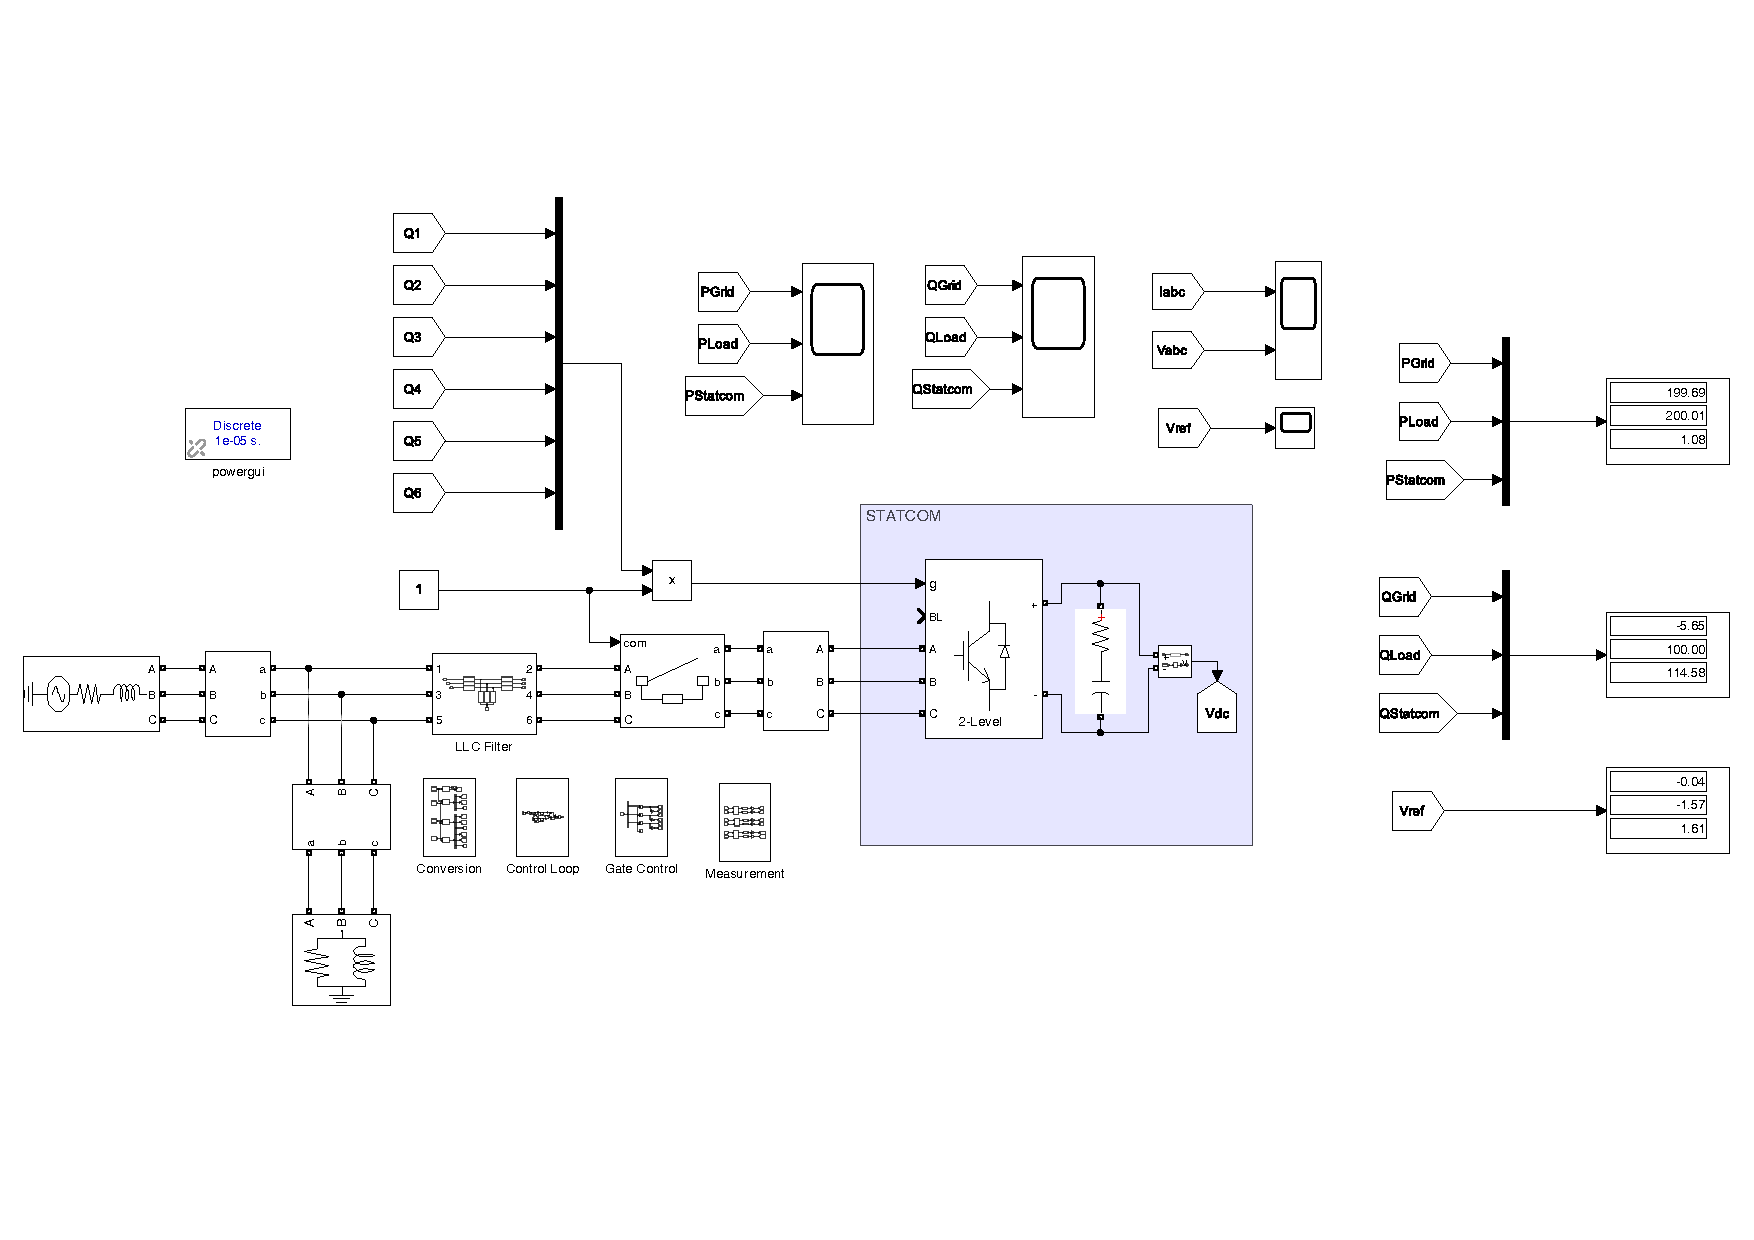
\includegraphics[page=1, width=\textwidth]{Full_Sys.pdf}
		\caption{Overall Architecture of the Grid-Connected STATCOM System.}
	\end{figure}
	
	\newpage
	% ---------------- SECTION 2: CONTROL STRATEGY ---------------- %
	\section{Control Strategy}
	The STATCOM's performance heavily relies on the Synchronous Reference Frame ($dq0$) control theory. This strategy transforms the three-phase time-varying AC signals ($abc$) into DC quantities ($dq0$) rotating at the synchronous speed, allowing the use of conventional Proportional-Integral (PI) controllers to achieve zero steady-state error.
	
	\subsection{Phase-Locked Loop (PLL) and Coordinate Transformation}
	A Three-Phase Phase-Locked Loop (PLL) continuously tracks the grid voltage to extract its phase angle ($\omega t$). As illustrated in Figure 2, this angle is fed into the $abc$-to-$dq0$ transformation blocks (Park's Transformation) to decompose the grid voltages, load currents, and STATCOM currents into active ($d$-axis) and reactive ($q$-axis) components. This decoupling enables independent control over the active power (which dictates the DC-link voltage) and the reactive power (which dictates the compensation level).
	
	\begin{figure}[H]
		\centering
		\includegraphics[page=3, width=0.55\textwidth]{Full_Sys.pdf}
		\caption{Coordinate Transformation Subsystem ($abc$ to $dq0$).}
	\end{figure}
	
	\newpage
	
	\subsection{Inner and Outer PI Control Loops}
	The control architecture is organized into cascaded loops, detailed in Figure 3:
	\begin{itemize}
		\item \textbf{Outer Voltage Loop:} Maintains the DC-link voltage at $800\text{V}$. The error between the measured $V_{DC}$ and the $800\text{V}$ reference is processed by a PI controller ($K_p = 5, K_i = 300$). The output of this loop represents the reference active current ($I_d^*$) required to replenish the converter's switching and conduction losses.
		\item \textbf{Inner Current Loops:} Two parallel PI controllers ($K_p = 25, K_i = 500$) regulate the $d$-axis and $q$-axis currents. The reactive current reference ($I_q^*$) is determined by the load's reactive power demand ($100\text{ kVAR}$) to ensure full compensation.
	\end{itemize}
	The outputs of the current controllers are transformed back to the $abc$ frame using the inverse Park transformation ($dq0$-to-$abc$) to form the modulating reference signals ($V_{ref}$).
	
	\begin{figure}[H]
		\centering
		\includegraphics[page=2, width=\textwidth]{Full_Sys.pdf}
		\caption{The $dq0$ Control Loop Subsystem showing PI controllers and Transformations.}
	\end{figure}
	
	\newpage
	\subsection{Sinusoidal Pulse Width Modulation (SPWM)}
	The continuous reference signals ($V_{ref}$) generated by the control loop are fed into the Gate Control subsystem (Figure 4). Here, they are compared against a high-frequency triangular carrier wave using relational operators. The carrier wave is implemented using a Repeating Sequence block configured for a time period of $100\,\mu\text{s}$, which translates to a precise $10\text{ kHz}$ switching frequency. The logic produces the necessary complementary gate pulses ($Q_1$ to $Q_6$) for the 6 IGBTs of the Two-Level VSC.
	
	\begin{figure}[H]
		\centering
		\includegraphics[page=4, width=0.5\textwidth]{Full_Sys.pdf}
		\caption{Gate Control Subsystem utilizing SPWM at 10 kHz.}
	\end{figure}
	
	\subsection{LCL Filter and Measurements}
	To interface the VSC with the grid, a third-order LCL filter is employed (Figure 5). This filter configuration gives stronger attenuation than a simple L-filter and reduces the $10\text{ kHz}$ switching components entering the AC grid (a THD measurement against a standard is not part of this study). Furthermore, the Measurement subsystem (Figure 6) utilizes first-order low-pass filters to process the instantaneous active and reactive power signals for smooth monitoring and analysis.
\begin{figure}[H]
	\centering
	\begin{subfigure}{0.48\textwidth}
		\centering
		\includegraphics[page=5, width=\textwidth]{Full_Sys.pdf}
		\caption{Three-Phase LCL Filter}
	\end{subfigure}
	\hfill
	\begin{subfigure}{0.48\textwidth}
		\centering
		\includegraphics[page=6, width=\textwidth]{Full_Sys.pdf}
		\caption{Measurement and Filtering Subsystem}
	\end{subfigure}
	\caption{Grid Interfacing Filter and Measurement Architecture.}
\end{figure}
	
	\newpage
	% ---------------- SECTION 3: SIMULATION RESULTS ---------------- %
	\section{Simulation Results and Analysis}
	The simulation was executed to validate the STATCOM's ability to maintain a unity power factor at the grid connection point by dynamically supplying the required reactive power.
	
	\subsection{Active and Reactive Power Flow}
	The most significant result is the power flow distribution among the Grid, Load, and STATCOM. As shown in Figure 7, the local load continuously demands $200\text{ kW}$ and $100\text{ kVAR}$. Once the STATCOM is engaged and reaches steady-state (after an initial transient period of approx. $0.2\text{ s}$), it injects precisely $100\text{ kVAR}$ (capacitive) into the point of common coupling (PCC). 
	
	Consequently, the grid is relieved from supplying reactive power ($Q_{Grid} \approx 0$), ensuring a unity power factor and minimizing transmission losses. The active power supplied by the grid is approximately the $200\text{ kW}$ load demand plus a small margin to sustain the STATCOM's internal switching losses.
	
	\begin{figure}[H]
		\centering
		\begin{subfigure}{0.75\textwidth}
			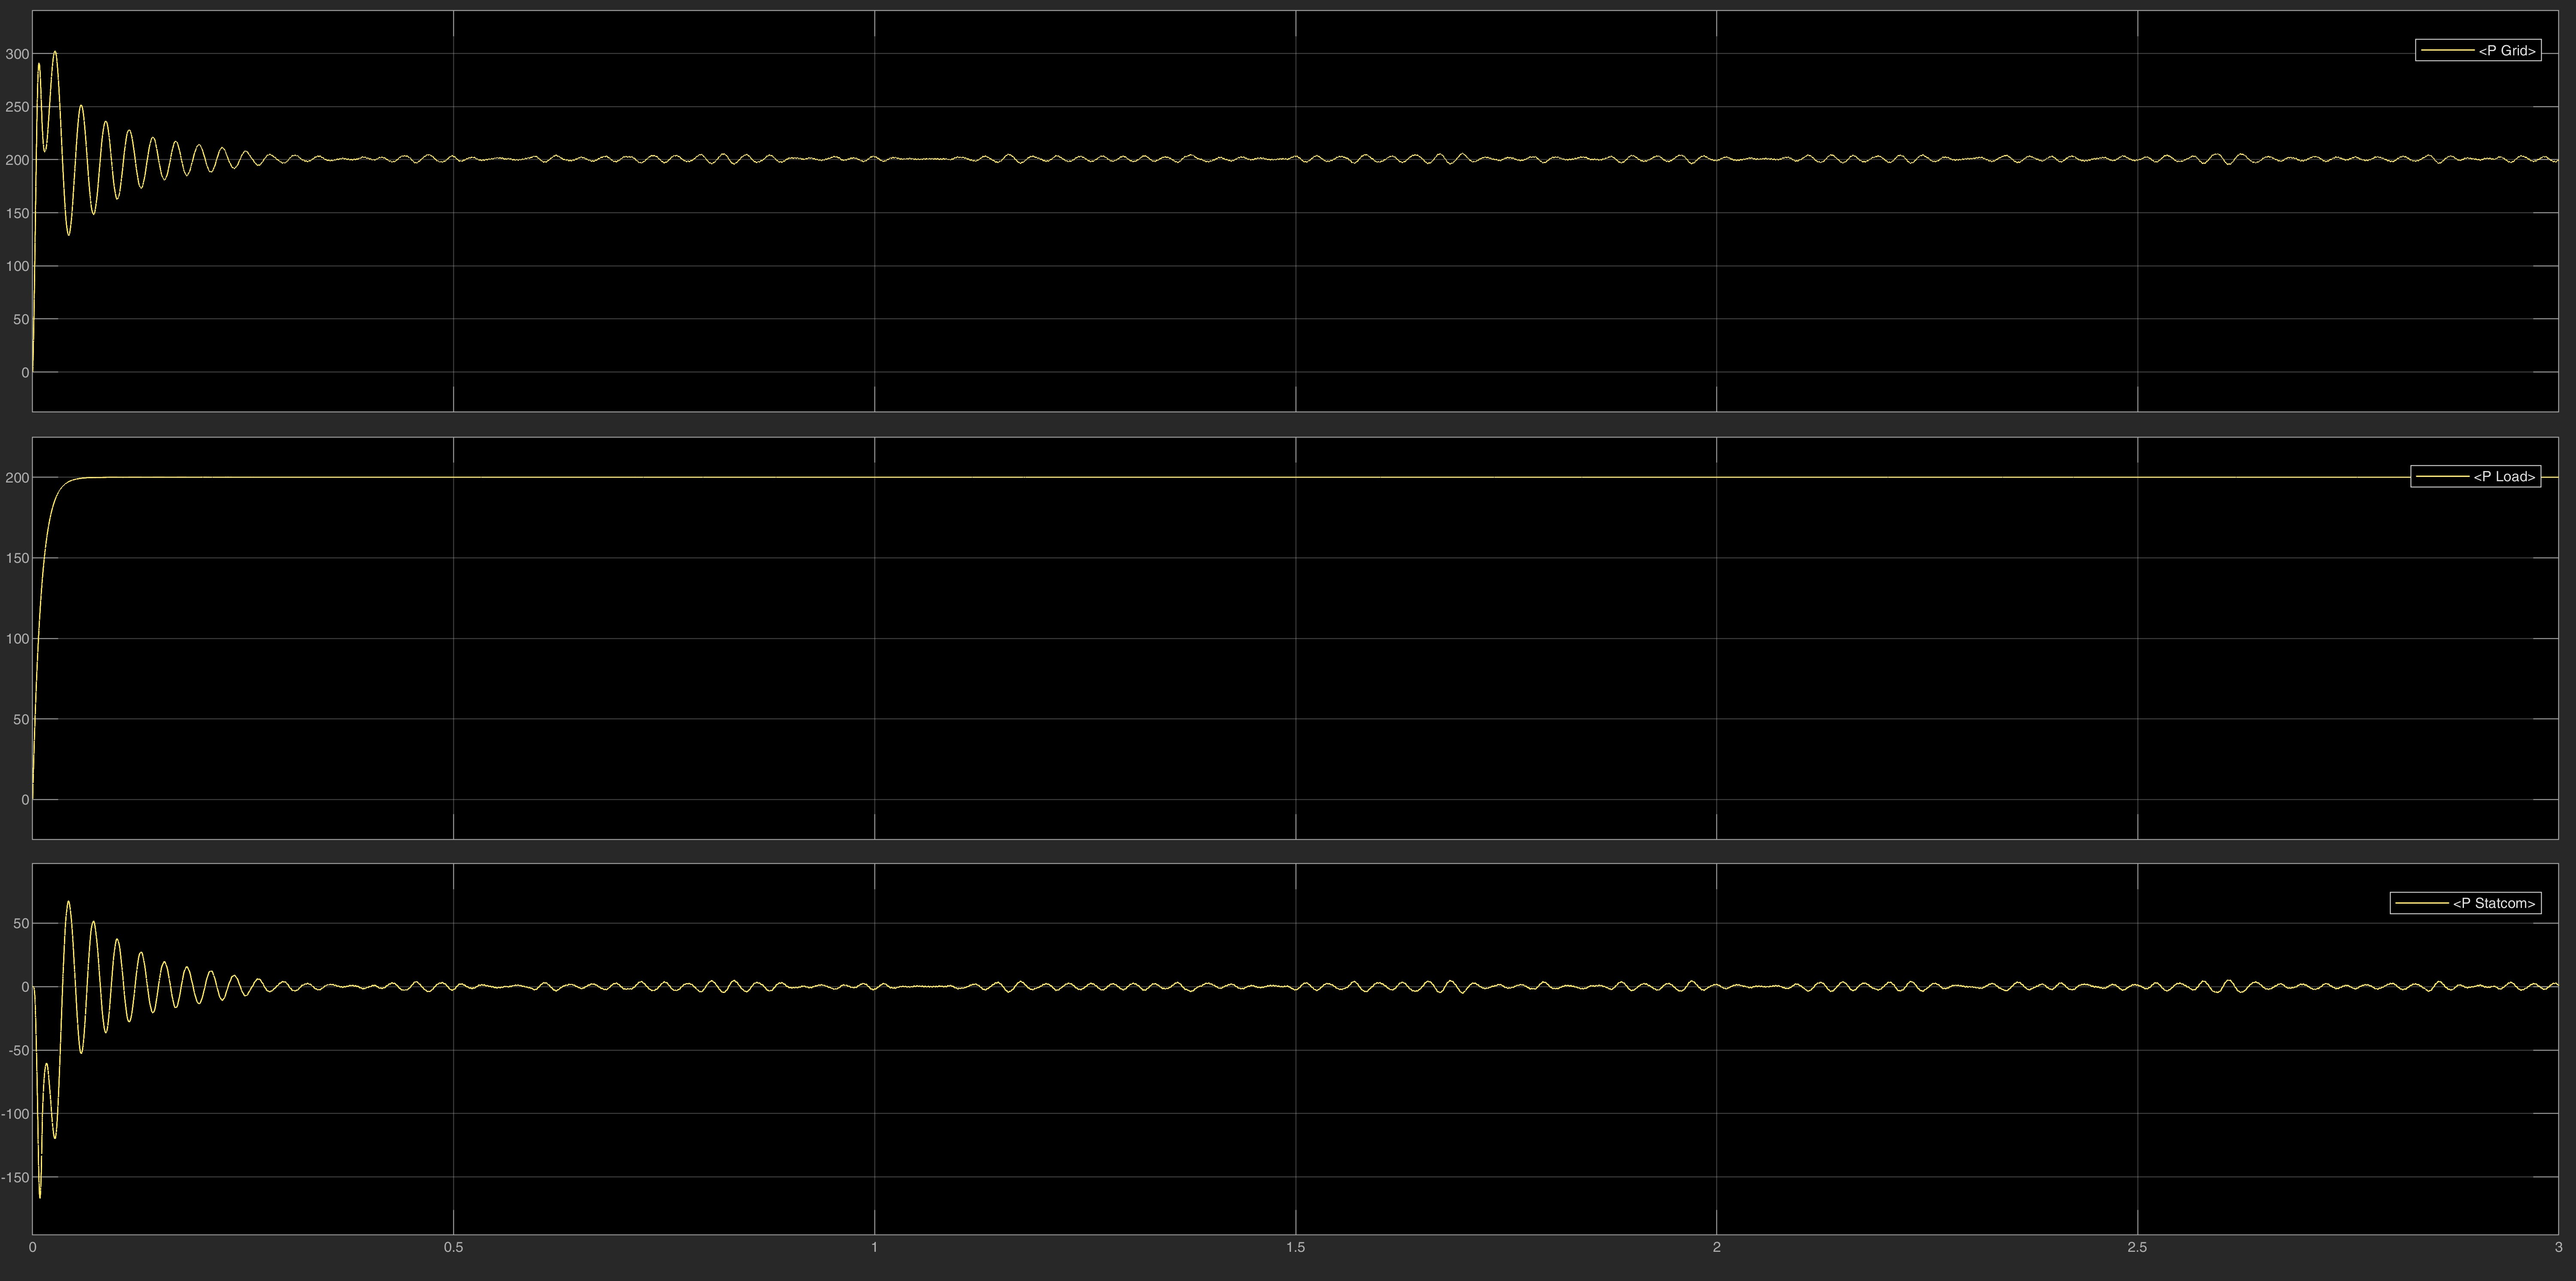
\includegraphics[width=\textwidth]{P_Scope1.jpg}
			\caption{Active Power Flow ($P$)}
		\end{subfigure}
		\vskip\baselineskip
		\begin{subfigure}{0.75\textwidth}
			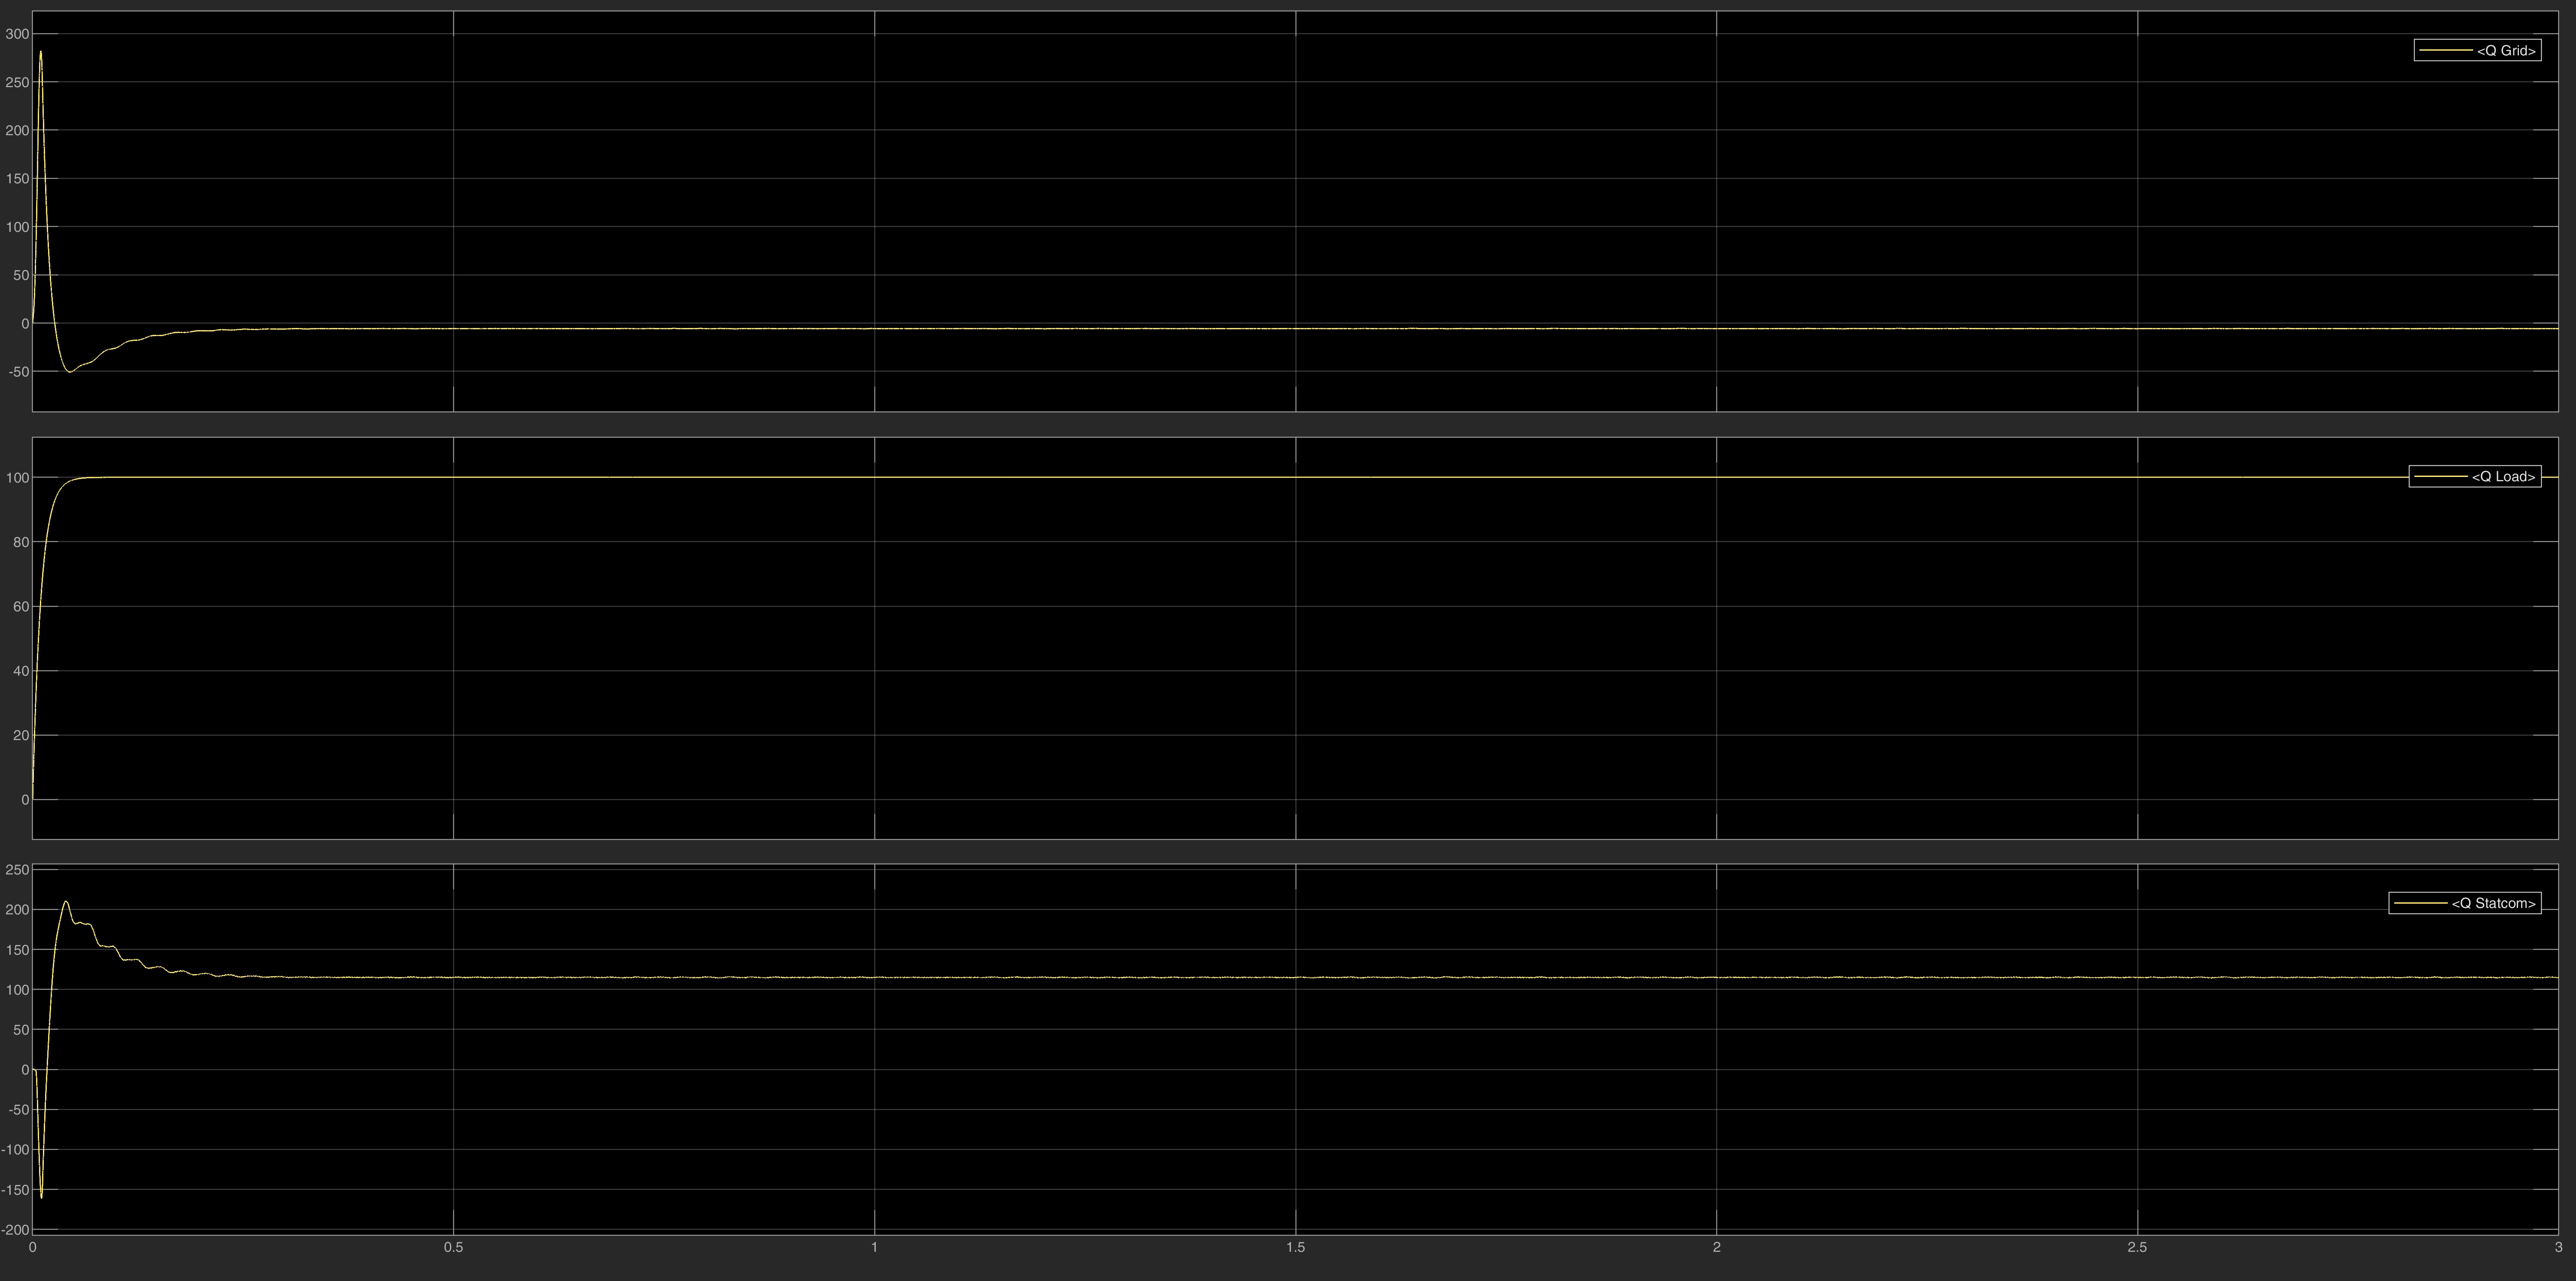
\includegraphics[width=\textwidth]{Q_Scope3.jpg}
			\caption{Reactive Power Flow ($Q$)}
		\end{subfigure}
		\caption{Power flow scopes demonstrating full reactive power compensation by the STATCOM.}
	\end{figure}
	
	\newpage
	\subsection{Current and Voltage Waveforms}
	Figure 8 displays the dynamic response of the system currents and the generated reference voltage. The currents exhibit a transient behavior during the startup phase ($0$ to $0.2\text{ s}$) as the DC-link charges and the PLL locks onto the grid frequency. After $0.2\text{ s}$, the system enters a stable steady-state operation. The LCL filter effectively attenuates the $10\text{ kHz}$ switching harmonics, resulting in sinusoidal currents.
	
	\begin{figure}[H]
		\centering
		\begin{subfigure}{0.75\textwidth}
			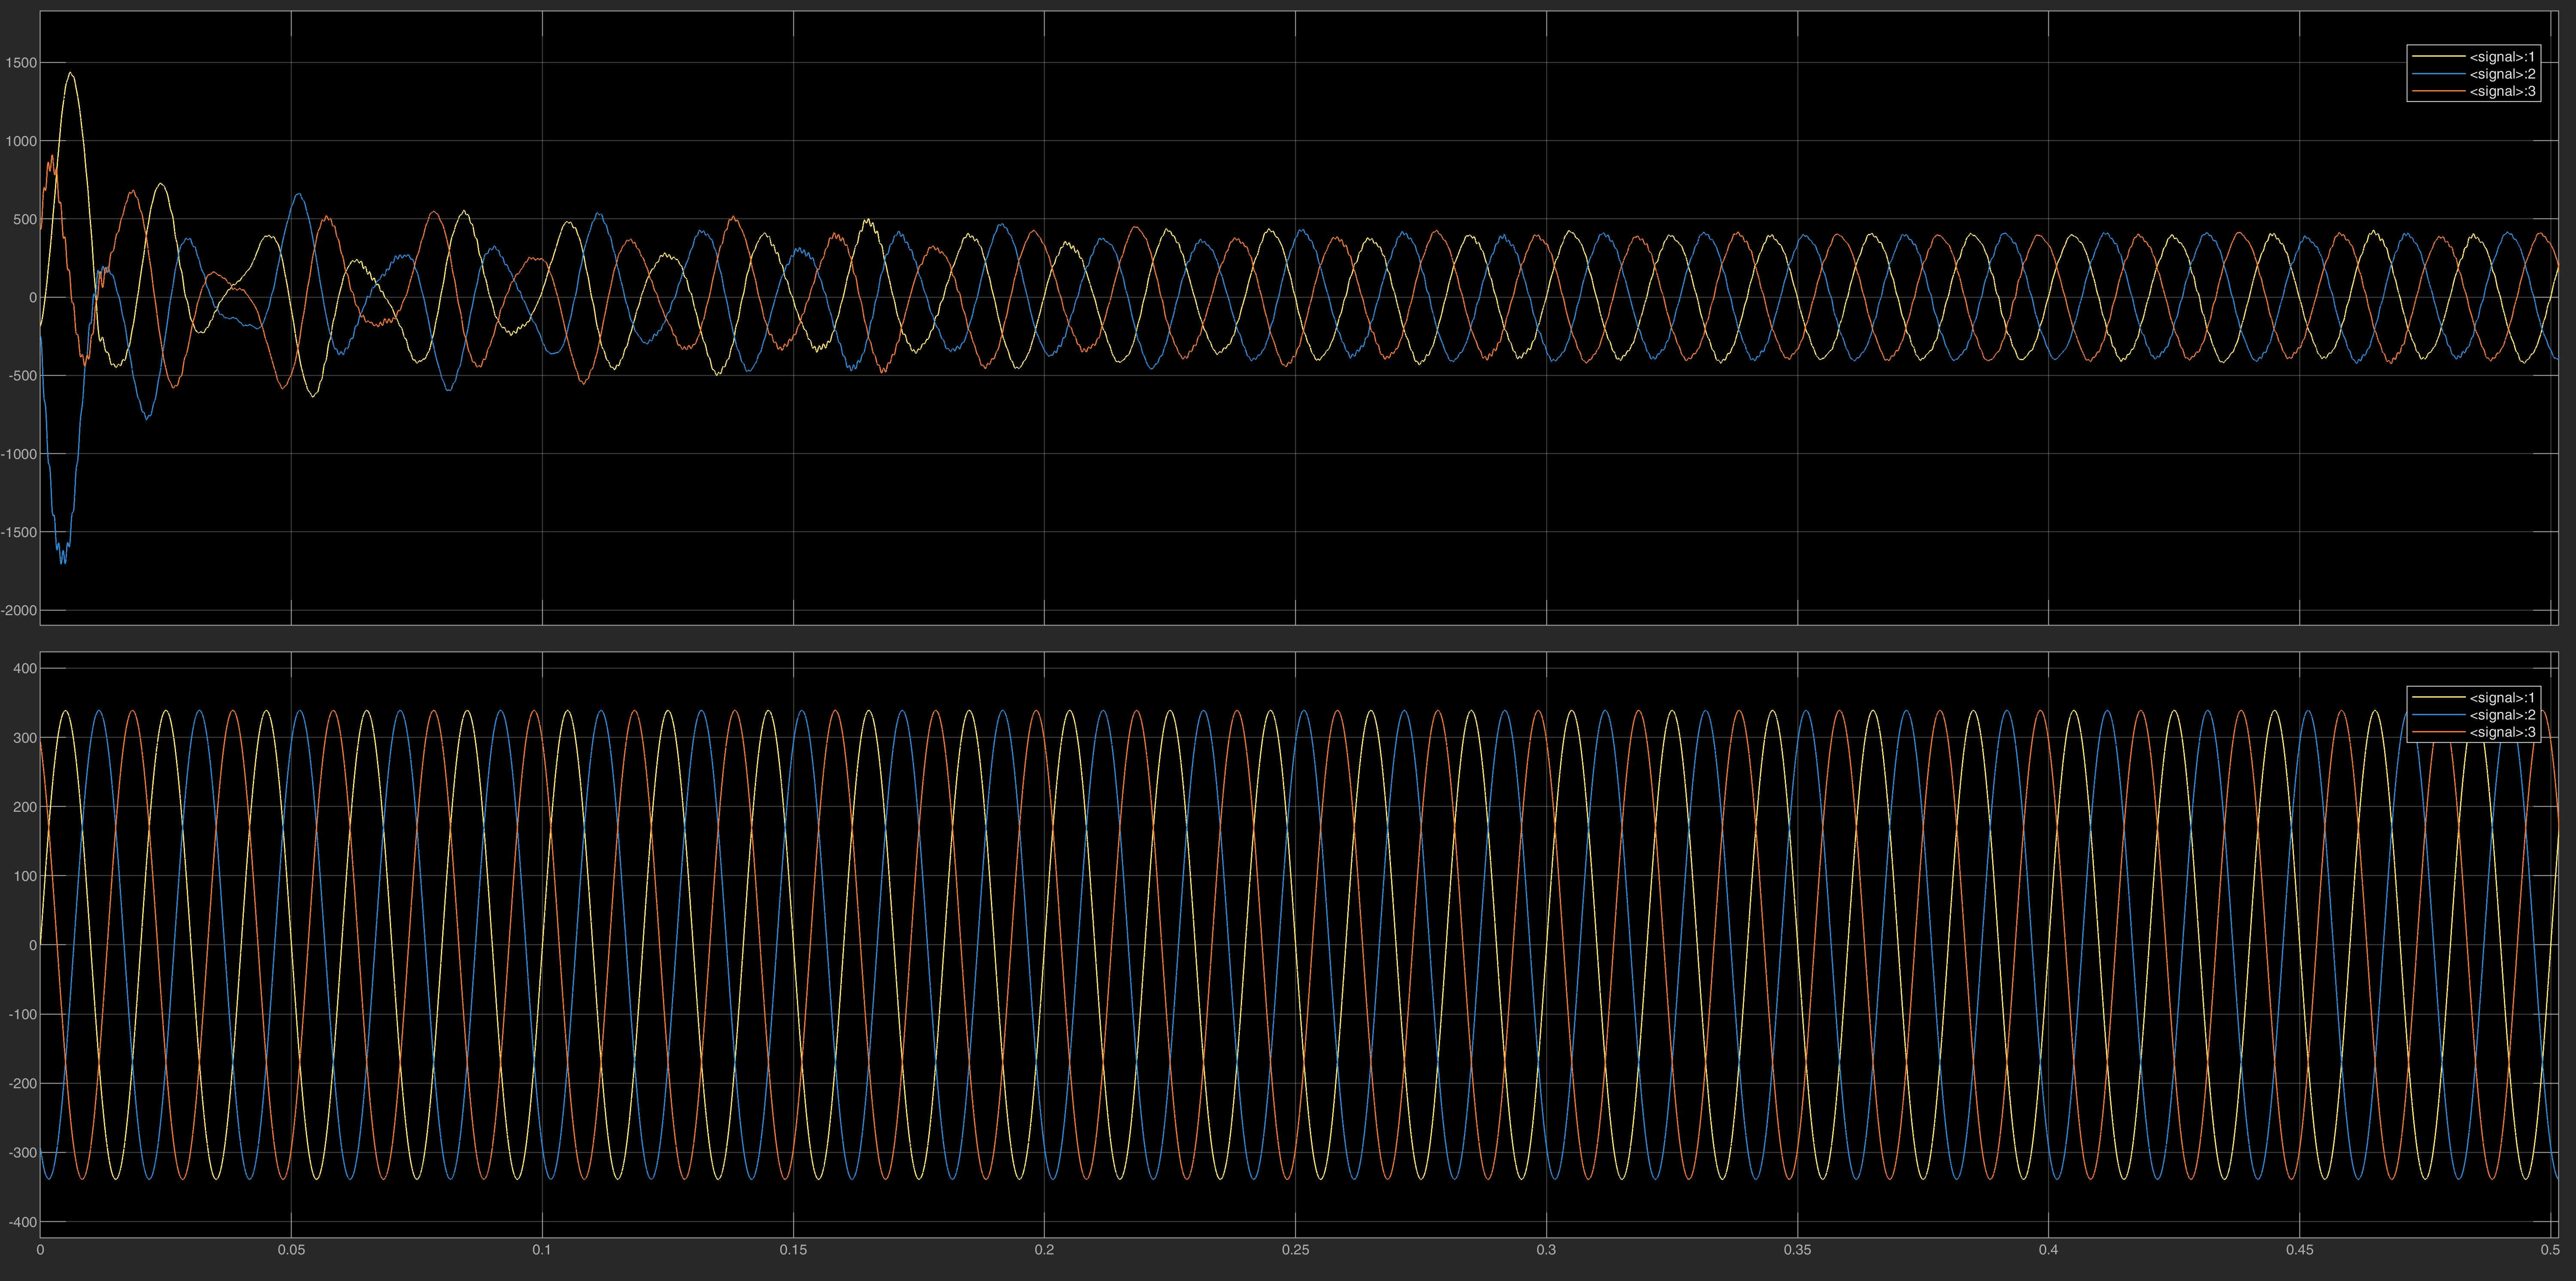
\includegraphics[width=\textwidth]{abc_Scope.jpg}
			\caption{Three-phase current waveforms for the Grid, Load, and STATCOM.}
		\end{subfigure}
		\vfill
		\begin{subfigure}{0.75\textwidth}
			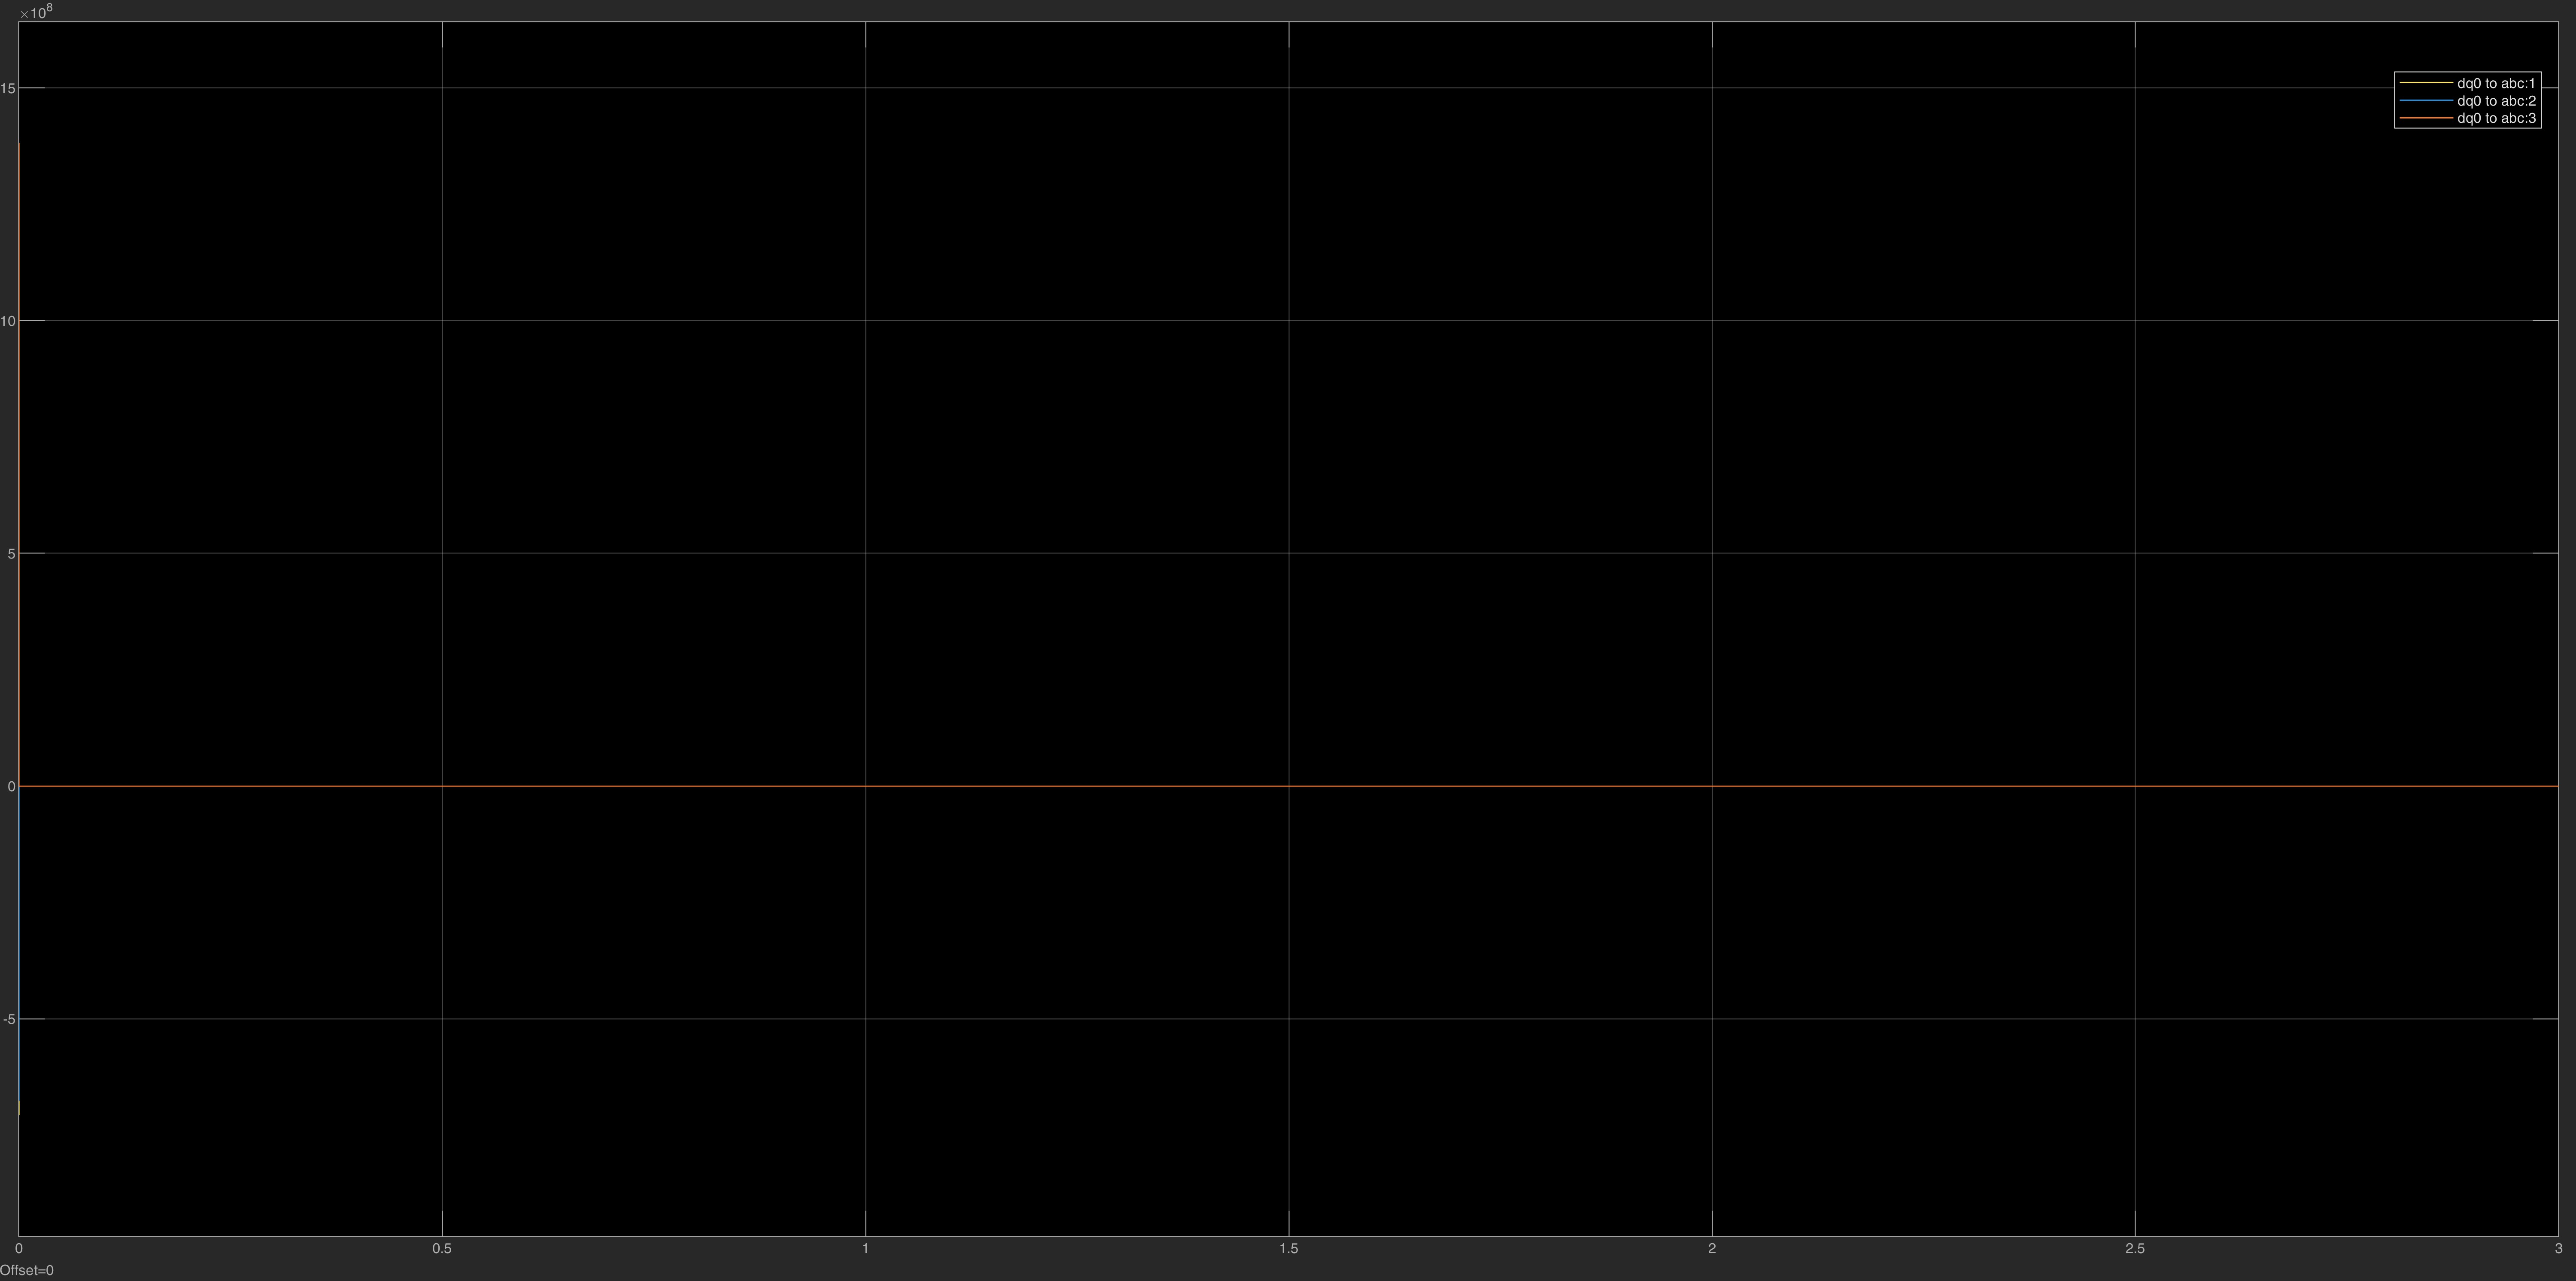
\includegraphics[width=\textwidth]{Vref_Scope2.jpg}
			\caption{Modulating reference signals ($V_{ref}$) generated by the controller.}
		\end{subfigure}
		\caption{Dynamic response of system currents and control signals.}
	\end{figure}
	
	\section{Conclusion}
	The design and simulation of the grid-connected STATCOM were carried out. The implementation of the $dq0$ Synchronous Reference Frame control allowed for precise, decoupled regulation of the DC-link voltage and reactive power. The STATCOM compensated the $100\text{ kVAR}$ inductive load demand, achieving a unity power factor at the grid side. The PI controller tuning gave a stable $800\text{ V}$ DC-link, and the high-frequency SPWM coupled with the LCL filter gave sinusoidal grid currents. This project solidifies the importance of flexible AC transmission systems (FACTS) in enhancing modern grid stability and efficiency.
	
\end{document}